\documentclass[main.tex]{subfiles}

\begin{document}

	\begingroup

	\renewcommand{\cleardoublepage}{}

	\renewcommand{\clearpage}{}

	\chapter{Clean Up Task Overview}

		\chapterauthor{Torge Olliges, Jan Schimpf, Jeremias Thun}
		
		\section{Goal}
		The goal of the Clean Up task is like the name indicates to clean a room. In the RoboCup several objects get distributed through out the room. The objects can be placed on the floor, tables or other furniture. Each of these objects is clearly visible and not hidden behind something. The task of the HSR is now to find these objects and place them into an designated basket. There exist multiple target positions and the HSR has to decide by itself the correct one based on the object. Like the Storing Grocery task the time limit is 5 minutes.

	  	\section{Tasks}
	  	The figure \ref{clean_up_seq_01} shows the procedure of Clean Up. The following subsections explain the execution and procedure in detail and give insights into the decisions made resulting in the exact plan depicted below. As well as for the Grocery Storing task, there will be a description of the most important sequences below.

	  	\begin{figure}	
	  		\centering
	  		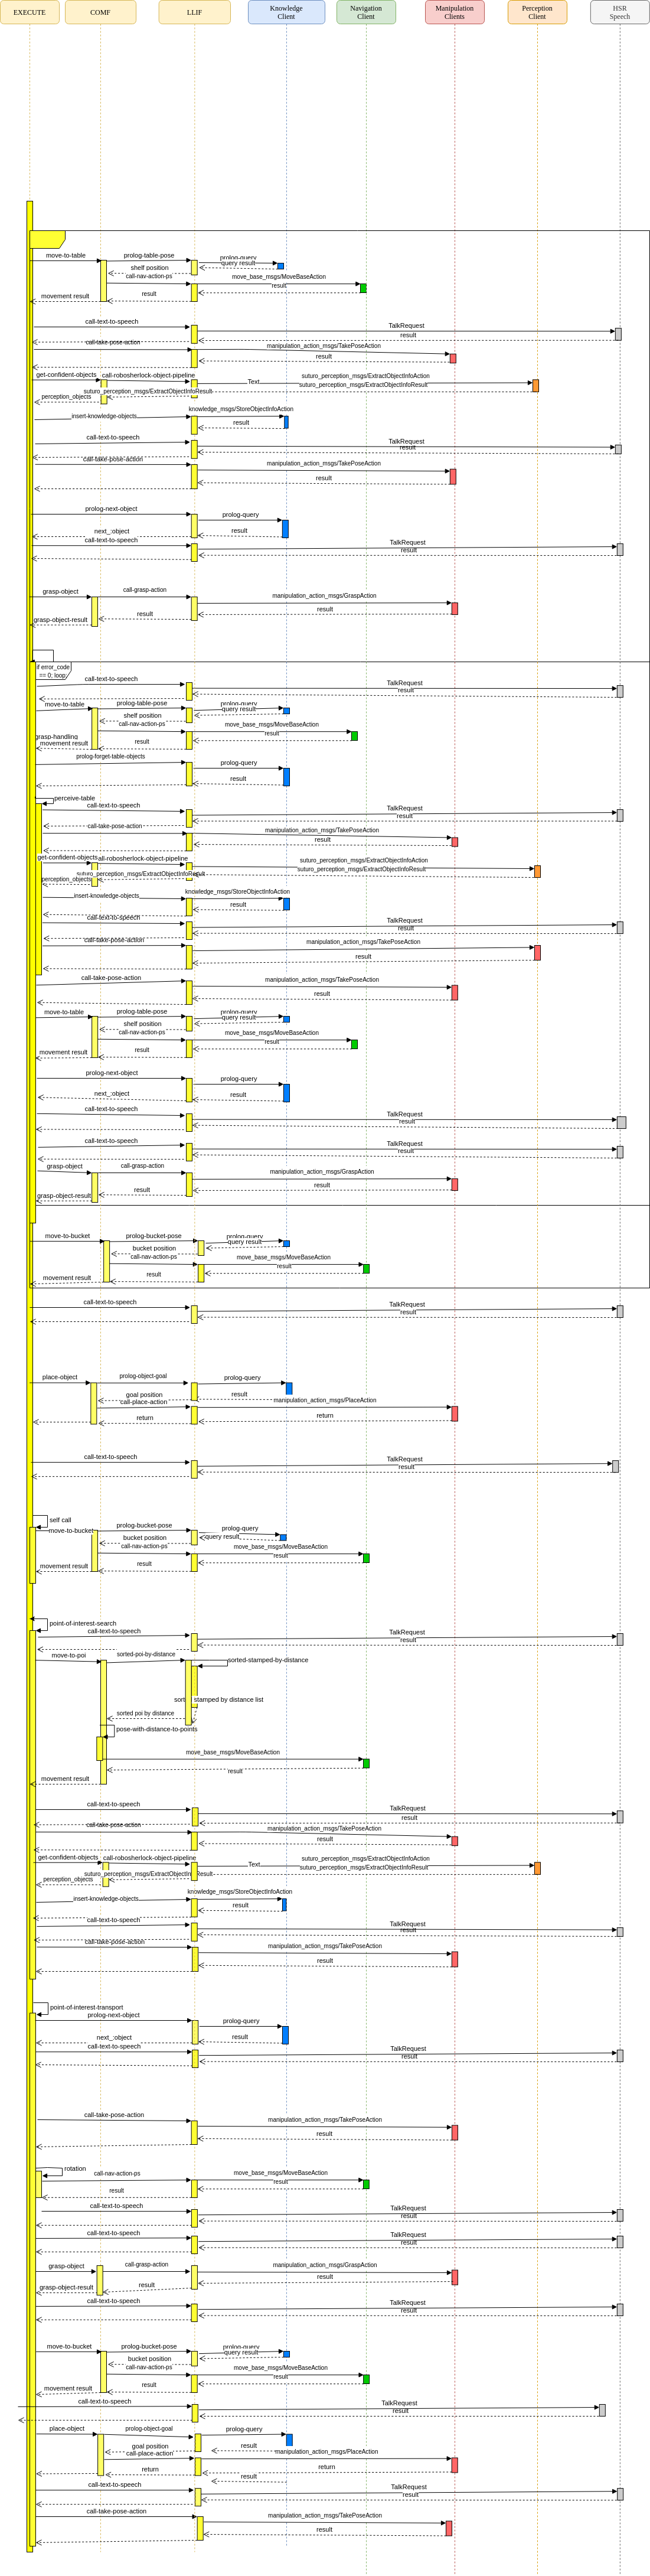
\includegraphics[width=0.85\textwidth]{pictures/diagramms/cleanup-sequence.png}
	  		\caption{Sequence diagram of the complete run of the clean up task \textit{(explanations below)}}
	  		\label{clean_up_seq_01}
	  	\end{figure}
	  	% TODO: Entfernen - hier bitte aus dem sequenz diagramm einen einzelnen task als subsection z.b. schritt: tür öffnen, dafür mussten perception dies tun manipulation das tun etc.
	  	
	\subsection{Setup}
	\begin{knowledge}	
	First the interface to Knowledge is called make the basket a \textit{target} surface and the floor and the table \textit{source} surfaces, since objects are picked up from both.
	\end{knowledge}
	
	% Manipulation: take pose action
	\begin{manipulation}
	Just as described in the task Grocery Storing, Manipulation needs to set the robot to the default pose.
	\end{manipulation}

	\subsection{Scan table sequence}
	
	% Knowledge: get table-poses
	\begin{knowledge}
	The Clean Up task starts by looking into the objects on the table(s), so Knowledge is needed to provide the position of the nearest table.
	\end{knowledge}
	
	% Navigation: moveBaseAction
	\begin{navigation}
	To perceive the table, the robot is again turned $90^\circ$ to the table. Allowing it to look over its shoulder having a clear view of the table.
	\end{navigation}
	
	% NLP
	\begin{nlp}
	Before the robot can actually start to perceive, the user will be informed by the computer voice, that the robot is now perceiving the table.
	\end{nlp}
	
	% Manipuilation: TakePoseAction
	\begin{manipulation}
	With the robot standing at the right spot, it is the task of Manipulation to get it into a position where it can perceive the table.
   \end{manipulation} 
	
	% Perception: Percieve and return data
	\begin{perception}
	In this position the table will be scanned an Percpetion again generates all necessary information about the objects standing on the table.
	\end{perception}
	
	% Knowledge: Store Data
	\begin{knowledge}
	As in the similar sequences in Grocery Storing, Knowledge stores the perceived data in the Knowledge base.
	\end{knowledge}
	% NLP: Talk Request
	
	% Manipulation: Take pose
	\begin{manipulation}
	To prepare for grasping, the robot is put back in its default position.
	\end{manipulation}
	
	% 2x NLP: Talk
	
	
	% Navigation: MoveBaseAction
	\begin{navigation}
	Also, the robot needs to be turned back from the perceiving pose by $90^\circ$ so it looks straight at the table and can grasp an object.
	\end{navigation}
	
	\subsection{Grasp sequence}\label{clean_up_grasp_seq}
	
	%prolog-next-object
	\begin{knowledge}
	Knowledge first decides which object to grasp first, which works the same way as in Grocery Storing and is purely based on the distance to the robot.
	\end{knowledge}
	
	%NLP Grasping object
	\begin{nlp}
	The computer voice of the robot is now informing everyone that the robot will now grasp an object. Right after that it also sayswhich object the robot will grasp based on the object id.
	\end{nlp}
	
	%grasp-object
	\begin{manipulation}
	The object id is used to query the Knowledge base for the dimensions of the object and the pose of the object. The results are then used to call the manipulation grasp server to grasp the object. Manipulation then gets the task to grasp the given object.
	\end{manipulation}
	 %Knowledge: prolog dimensions
	 %Knowledge: prolog pose
	 \begin{knowledge}
	 Knowledge again realizes that the gripper now carries an object and attaches that object to the gripper in the Knowledge base.
	 \end{knowledge}
	 
	%NLP succesfully grasped
	\begin{nlp}
	Grasping the object is completed by the robot saying that it has successfully grasped the object.
	\end{nlp}
    
	\subsection{Place sequence}
	%Navigation: moveBaseAction
	The robot moves to the designated location in this case the bucket.
	The coordinates for the navigation call are queried from the Knowledge base and adjusted so the robot looks at the bucket and can place the object inside it. 
	
	%NLP placing the object
	Informing that the robot is now placing the object

	%place-object
	The object id is used to query the Knowledge base for the dimensions of the object and the goal of the object. The results are then used to call the manipulation place server to place the object. Manipulation then gets the task to place the previously grasped object in the given destination. To do that the Place Action Server has to calculate the correct orientations to place from the right direction and do collision avoidance with all other objects which is done by using \textit{Giskard}.
	 %Knowledge: prolog dimensions
	 %Knowledge: prolog goal
	 
	%NLP placed the object
	Informing that the robot has successfully placed the object

	%Manipulation: Take pose
	Returns the robot into the default pose.
	
	This is looped for two times.
	The first one is for the table and stops if there are no more objects on it to be placed in the bucked. The sedon one is for the point of interest search and stops if there are not points of interest left.
	
	\subsection{Point of interest search sequence}
	The object finder node publishes a list of poses that may be an object. This list will from now on be called points of interests.
	
    %NLP found an point of interest to search
    Informing that the robot has found a point of interest to search for objects
    
    %move-to-poi
    The first pose of the points of interest is taken. A target position is calculated that enables the HSR to perceive the position. This target pose is then send to navigation and executed.
    
    %call-take-pose-action
    The HSR is brought into the perceive pose for the floor.
    
    %NLP perceiving the postition
    Informing that the robot is now perceiving the position
      
    %call-robosherlock-object-pipeline
	The HSR takes a picture of the scene it is currently looking at and processes it with \textit{RoboSherlock}. Based on the requested region the input images are filtered. The results are then published by the \textit{perception\_actionserver}.

    
    %Knowledge:insert-knowledge-objects
    Knowledge checks the data of the objects, that are supposed to be stored. If the class of an object is unknown to Knowledge, it is set to other. If the data for the given object is valid, the object gets added to the Knowledge base. Should other objects be close to the new one, they get organized in a group. Groups are used to sort objects and can be used to determine if an object is hard to grasp.
    
    %call-take-pose-action
   	Returns the robot into the default pose to be able to grasp the object.

    % Navigation: MoveBaseAction
    Turn the HSR by $90^\circ$ so he can grasp objects which would not be possible from the pose he took to perceive the objects.

    The plan continues from the \ref{clean_up_grasp_seq}.
    
    
	\section{Conclusion}
	The Clean Up task was still incomplete for the test robocup and wasn't executed due to having various problems getting the robot to run in the challenge room, but was in a executable and working state for the third milestone demo and successfully completed the demo run. During this run it showed that the tasks grasping the objects of the table or from the floor, transporting the objects and placing them in the basket were achieved in the simulation.\\
	Even with the run being successfully completed the plan has similar problems to the Grocery Storing task with the magnet sensors and there are still potential issues as the way items on the floor are currently searched for involves the laser scanner so items that are to small to be picked up by the laser scanner won't be found by the robot.\\
	Overall the Clean Up task can be considered as an success as all the necessary tasks that are part of the Clean Up challenge can be completed. 
	
	\endgroup

\end{document}
